% DO NOT COMPILE THIS FILE DIRECTLY!
% This is included by the other .tex files.

\begin{frame}[t,plain]
\titlepage
\end{frame}




\begin{frame}[t]{Obtención de IP}

\textbf{Utilizar ping en CMD}

\begin{wrapfigure}{r}{0.43\textwidth} 
\vspace{2pt}
  \begin{center}
    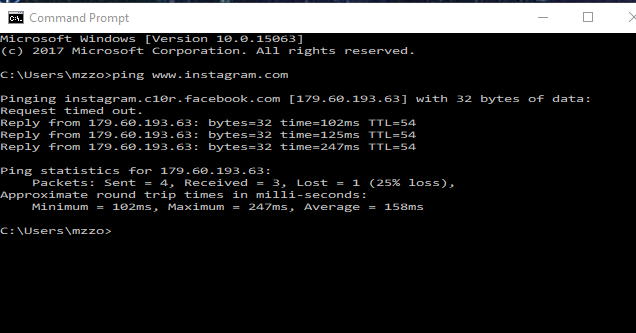
\includegraphics[width=0.48\textwidth]{pinginstagram.png}
    \label{fig:databaseUserTable}
  \end{center}
  \vspace{2pt}
\end{wrapfigure} 

\bigskip

Por medio de la consola predispuesta por windows y el uso de la url \emph{www.instagram.com}, se realiza un diagnostico de la determinada red, con el fin de conseguir su respectiva IP. 
Entonces se utiliza:

\begin{center}
   \textbf{ping www.instagram.com}
\end{center}

se obtiene

\begin{center}
   \textbf{179.60.193.63}
\end{center}





\end{frame}



\begin{frame}[t,fragile]{Herramientas}

\textbf{Metasploit}

\begin{wrapfigure}{r}{0.43\textwidth} 
\vspace{2pt}
  \begin{center}
    
\includegraphics[width=0.5\textwidth]{meta.jpg}
    \label{fig:databaseUserTable}
  \end{center}
  \vspace{2pt}
\end{wrapfigure} 

\bigskip

 Herramienta  utilizada para desarrollar y ejecutar exploits contra una máquina remota, generando scripts de utilidad, declarando ejercicios como DoS u otros, de tal manera de generar pruebas dentro de la IP obtenida.


\end{frame}

\begin{frame}[t,fragile]{Herramientas}

\textbf{Lineas de Comando}

\begin{wrapfigure}{r}{0.43\textwidth} 
\vspace{2pt}
  \begin{center}
    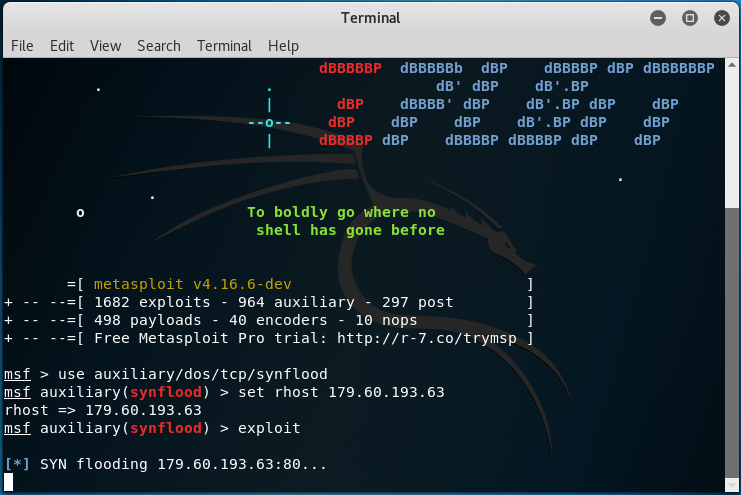
\includegraphics[width=0.45\textwidth]{sploit.png}
    \label{fig:databaseUserTable}
  \end{center}
  \vspace{2pt}
\end{wrapfigure} 

\bigskip

Se dispone a utilizar el siguiente comando \textbf{use auxiliary/dos/tcp/synflood}, donde se provee \textbf{auxiliary}, el cual permite la obtención de información sobr el objetivo, con tal de determinar las posibles vulnerabilidades. Además de proveer el protocolo \textbf{tcp} y  el tipo de ataque a realizar, el cual para este caso corresponde a \textbf{dos} y \textbf{synflood} 

\end{frame}

\begin{frame}[t,fragile]{Herramientas}

\textbf{Lineas de Comando}

\bigskip

Finalmente se setea el \textbf{rhost} ligado a la IP \textbf{179.60.193.63} para finalmente ejecutar el exploit generado.

\begin{figure}[!h]
    \centering
    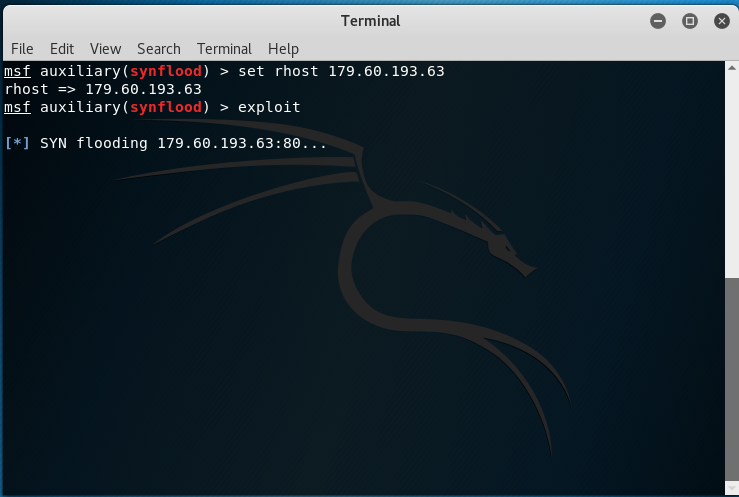
\includegraphics[scale=0.35]{metaesploit.png}
    \label{fig:my_label}
    \end{figure}

\end{frame}



\begin{frame}[t,fragile]{Herramientas}

\textbf{Wireshark}

\bigskip

A continuación se da a conocer una vista del envio de paquetes al realizar el exploit mencionado anteriormente.

\begin{figure}[!h]
    \centering
    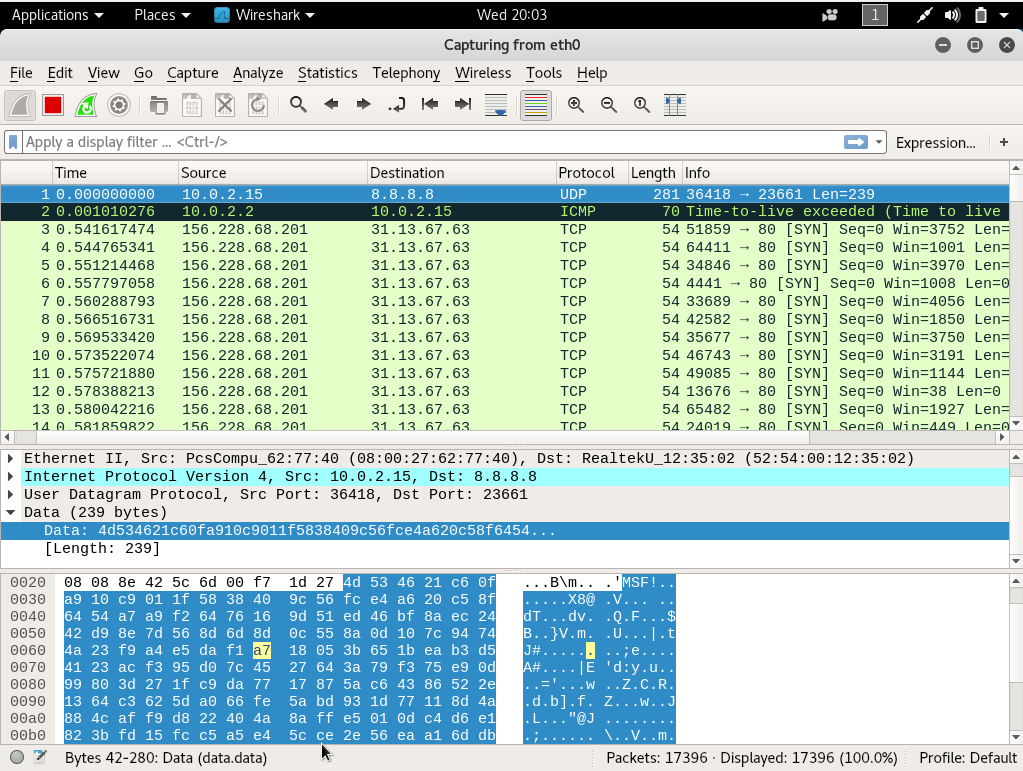
\includegraphics[scale=0.25]{wireshark.png}
    \label{fig:my_label}
    \end{figure}

\end{frame}



